\documentclass[11pt,a4paper]{article}

\usepackage[T1]{fontenc}
\usepackage[utf8]{inputenc}
\usepackage{lmodern}
\usepackage{microtype}
\usepackage{geometry}
\usepackage{graphicx}
\usepackage{booktabs}
\usepackage{amsmath,amssymb}
\usepackage{xcolor}
\usepackage{tikz}
\usetikzlibrary{positioning}
\usepackage{hyperref}
\usepackage{cleveref}
\usepackage[backend=biber,style=authoryear]{biblatex}
\addbibresource{references.bib}

\geometry{margin=1in}
\title{LaTeX PDF Pipeline — End-to-End Test Document}
\author{Pipeline Test Fixture}
\date{\today}

\begin{document}
\maketitle
\tableofcontents

\section{Purpose}\label{sec:purpose}
This document is a small but realistic end-to-end fixture for the repository's LaTeX CI/CD pipeline. It tests a master document, chapter inputs, mathematics, tables, graphics, cross-references, and a BibLaTeX bibliography.

\section{Multi-file input}\label{sec:multifile}
The master document loads two chapter files with \verb|\input|. See \cref{sec:math} for the mathematics example and \cref{fig:pipeline} for the generated figure.

\section{Mathematics}\label{sec:math}
A displayed equation checks that the mathematics packages are available:
\begin{equation}\label{eq:quadratic}
  f(x)=ax^2+bx+c, \qquad a\ne0.
\end{equation}
Equation~\cref{eq:quadratic} is a standard quadratic polynomial. The chapter is intentionally separate from the master file to test relative input resolution.

\section{Tables and Lists}\label{sec:data}
The table below checks common table support.

\begin{table}[htbp]
\centering
\caption{Sample pipeline checks}
\label{tab:checks}
\begin{tabular}{lll}
\toprule
Component & Check & Expected result \\
\midrule
TeX source & Parse & Success \\
Bibliography & Biber & Success \\
Cross-reference & Resolve & Success \\
PDF output & Artifact & Present \\
\bottomrule
\end{tabular}
\end{table}

As shown in \cref{tab:checks}, the fixture covers the core compilation stages.

\begin{itemize}
  \item Master \texttt{.tex} file
  \item Multiple chapter inputs
  \item Bibliography database
  \item Cross-references
  \item Mathematics and tables
  \item TikZ-generated graphics
\end{itemize}


\section{Generated graphic}\label{sec:figure}
Figure~\cref{fig:pipeline} is generated entirely with TikZ, so the fixture has no external binary image dependency.

\begin{figure}[htbp]
  \centering
  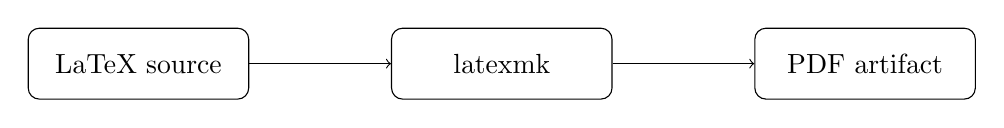
\begin{tikzpicture}[node distance=18mm, every node/.style={draw, rounded corners, align=center, minimum width=28mm, minimum height=9mm}]
    \node (tex) {LaTeX source};
    \node (latexmk) [right=of tex] {latexmk};
    \node (pdf) [right=of latexmk] {PDF artifact};
    \draw[->] (tex) -- (latexmk);
    \draw[->] (latexmk) -- (pdf);
  \end{tikzpicture}
  \caption{Minimal pipeline flow used by this test fixture.}
  \label{fig:pipeline}
\end{figure}

\section{Bibliography}\label{sec:bib}
A bibliography entry is cited here to exercise the Biber path: \parencite{lamport1994}.

\printbibliography

\end{document}
